\documentclass[11pt,a4paper]{article}

% Get the necessary packages for the document.
% Set to english language and utf8.
\usepackage[english]{babel}
\usepackage[utf8]{inputenc}

% Some packages for symbols we need within the tutorial.
\usepackage{dingbat}
\usepackage{marvosym}

% For the sourcecode.
\usepackage{listings}

% For the links etc.
\usepackage[pdfborder={0 0 0}]{hyperref}

% For the pdf-graphics.
\usepackage{graphicx}

% The steamroller tactics to fix figures and so on.
\usepackage{float}

% This is for tables which are to long to be shown on one page.
\usepackage{longtable}

% This package is for the directory tree structures
\usepackage{dirtree}

% We need this package for some color within the document.
\usepackage{color}

% This is the package for the margin-nodes.
\usepackage[color=white, bordercolor=white]{todonotes}

\usepackage{amsfonts}
\usepackage{setspace}
\usepackage{ae,aecompl}

\usepackage[automark]{scrpage2}

\usepackage[margin=0.5cm,indention=-3em,font={sf},labelfont={bf,sf},format=hang]{caption}
% Get the new commands we defined for this document.
% The name of Kieker, just for the case that the design of this should change.
\newcommand{\Kieker}{\textsf{Kieker}}

% The current version-string.
\newcommand{\version}{1.5-trunk}

% The single parts of Kieker and some files.
\newcommand{\KiekerMonitoringPart}{\textsf{Kieker.Monitoring}}
\newcommand{\KiekerAnalysisPart}{\textsf{Kieker.Analysis}}
\newcommand{\analysisJar}{kieker-analysis-\version.jar}
\newcommand{\monitoringJar}{kieker-monitoring-\version.jar}
\newcommand{\commonJar}{kieker-common-\version.jar}
\newcommand{\toolsJar}{kieker-tools-\version.jar}
\newcommand{\commonsLoggingJar}{commons-logging-1.1.1.jar}
\newcommand{\monitoringPropertiesFile}{kieker.monitoring.properties}
\newcommand{\analysisPropertiesFile}{kieker.analysis.properties}
\newcommand{\logFourJPropertiesFile}{log4j.properties}
\newcommand{\aopFile}{aop.xml}

% The complete url where to find Kieker.
\newcommand{\KiekerURL}{\url{http://sourceforge.net/projects/kieker/files}}

% This is how we call the kieker directory.
\newcommand{\KiekerDir}{kieker-\version{}}%{$<$KIEKER-DIR$>$}

% These commands are necessary to mark classes, methods and files within the document.
\newcommand{\class}[1]{\texttt{#1}}
\newcommand{\method}[1]{\textit{#1}}
\newcommand{\dir}[1]{\texttt{#1}}
\newcommand{\file}[1]{\texttt{#1}}

% TODO command for our document
\newcommand{\TODO}[1]{\todo[inline,color=green!40]{TODO: #1}}

% These commands are for notifying the reader about something important.
\newcommand{\marginbox}[1]{\todo[noline]{#1}}
\newcommand{\notify}{\marginbox{\huge{\rightpointleft}}}
\newcommand{\warning}{\marginbox{\huge{\Stopsign}}}


% The following commands set the listings for the different (programming) languages correctly.
% For the first they use all nearly the same settings.
\newcommand{\setListing}[4]{
\lstset{
language=#1,          
numbers=#2,
basicstyle=#3,       	% the size of the fonts that are used for the code
showspaces=false,               % show spaces adding particular underscores
showstringspaces=false,         % underline spaces within strings
showtabs=false,                 % show tabs within strings adding particular underscores
%frame=shadowbox,	                % adds a frame around the code
frame=lrtb,
rulesepcolor=\color{black},
tabsize=2,	                % sets default tabsize to 2 spaces
captionpos=t,                   % sets the caption-position to bottom
breaklines=true,                % sets automatic line breaking
breakatwhitespace=false,        % sets if automatic breaks should only happen at whitespace
title=\lstname,                 % show the filename of files included with \lstinputlisting; also try caption instead of title
escapechar={#4}
}
}
\newcommand{\setJavaCodeListing}{\setListing{Java}{left}{\sffamily\scriptsize}{}}
\newcommand{\setBashListing}{\setListing{Bash}{none}{\sffamily\scriptsize}{°}}
\newcommand{\setXMLListing}{\setListing{XML}{none}{\sffamily\scriptsize}{}}


\title{Kieker Data Bridge}
\author{Reiner Jung}
\date{\today}

\begin{document}

\maketitle

\tableofcontents

%%
\section{Introduction}  

% Why Kieker Data Bridge
Kieker is a Java-centric monitoring framework. To open Kieker for other language platforms and technologies, specific extensions have been developed for Visual Basic 6, .Net or Cobol. However, each extension reimplemented features which have to be maintained for every Kieker release. This fostered the idea to provide a common platform and design model for additional extension to minimize the effort necessary to integrate new languages and technologies.

The Kieker Data Bridge (KDB) is designed to provide this common platform. The KDB supports different sources of monitoring records and is embeddable in other tools such as Eclipse. In general the KDB receives records online through a connector, converts them to Kieker \texttt{IMonitoringRecord}s and serializes them with a Kieker writer.

In the following, the overall design and architecture is explained in Section~\ref{s:design}. Section~\ref{s:using-kdb} provides basic information on the command line version of the KDB. Section~\ref{s:extension} illustrates the extension of the KDB. And Section~\ref{s:outlook} explains the future development.

%%
\section{Design and Architecture}\label{s:design}

The internal architecture of the KDB uses an inversion of control pattern, where a \texttt{ServiceContainer} handles the processing of received records and steers Kieker to serialize the data. The container requires a service connector implementing the \texttt{IServiceConnector} to de-serialize records from information sources. The general architecture is illustrated in \autoref{fig:kdb-arch}

\begin{figure}[htb]
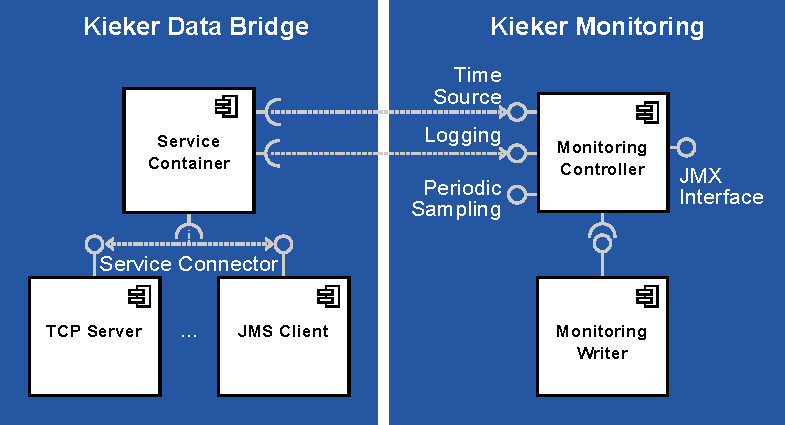
\includegraphics[width=\textwidth]{images/kieker-data-bridge.pdf}
\caption{General Kieker Data Bridge (KDB) architecture}
\label{fig:kdb-arch}
\end{figure}

The \texttt{IServiceConnector} interface has three methods:

\begin{itemize}
\item \texttt{initialize()} which initializes a remote connection
\item \texttt{close()} which terminates the connection
\item \texttt{deserializeNextRecord()} which receives one new record
\end{itemize}

\noindent
The \texttt{initialize()} method may block until the connection is established or an error occurs. However, it can also be implemented in a non-blocking way. The \texttt{deserializeNextRecord()} method must be blocking until a record is received, an error occurs, or the connection is terminated.

The \texttt{ServiceContainer} comprises of a constructor and six service methods. The constructor requires a Kieker-configuration, a connector and a respawn flag. The latter flag is a debatable construct, but is allows to trigger reconnects for simple connectors. It might be removed in future versions of the bridge.

%%
\section{Using Kieker Data Bridge}\label{s:using-kdb}

The KDB comes with a command line server including the bridge with a wide set of parameters:

\begin{lstlisting}[caption=Command line options of the Kieker Data Bridge]
usage: cli-kieker-service [-c <configuration>] [-d] 
       [-h <hostname>] -L <paths> [-l <jms-url>] -m
       <map-file> [-p <number>] [-s] -t <type>
       [-u <username>] [-v <arg>] [-w <password>]
 --c,--configuration <configuration>
        kieker configuration file

 --d,--daemon
        detach from console; TCP server allows multiple 
        connections

 --h,--host <hostname>
        connect to server named <hostname>

 --L,--libraries <paths>
        List of library paths separated by :

 --l,--url <jms-url>
        URL for JMS server

 --m,--map <map-file>
        Class name to id (integer or string) mapping

 --p,--port <number>
        listen at port (tcp-server or jms-embedded) or
        connect to port (tcp-client)

 --s,--stats
        output performance statistics

 --t,--type <type>
        select the service type: tcp-client,
        tcp-server, tcp-single-server, 
        jms-client, jms-embedded

 --u,--user <username>
        user name for a JMS service

 --v,--verbose <arg>
        output processing information

 --w,--password <password>
        password for a JMS service
\end{lstlisting}

\noindent
In addition the connectors can be initialized via a Configuration object determined by the \texttt{-c} option.

%
\subsection{Connectors}

The KDB supports presently five different connectors which are described here briefly. The selection of the connector can by done via the \texttt{--type} property on command line or via a Kieker-configuration file entry:

\begin{verbatim}
kieker.tools.bridge.connector=FullQualifiedClassName
\end{verbatim}

%
\subsubsection{TCPClientConnector}

Connects to a remote site specified by a host name and a port. The connector reads then binary data and reconstructs records. The two configuration properties can either be specified as a command line option or via the Kieker-configuration file by:

\begin{verbatim}
kieker.tools.bridge.connector.tcp.TCPClientConnector.hostname=HOSTNAME
kieker.tools.bridge.connector.tcp.TCPClientConnector.port=PORT
\end{verbatim}

%
\subsubsection{TCPSingleServerConnector}

Sets up a server for a single connection in \texttt{initialize()} and waits for a connection. After the connections is established the method terminates, and the \texttt{ServiceContainer} calls repeatedly the \texttt{deserializeNextRecord} method. The connector requires a port number for its port. The configuration property can either be specified by a command line option or via the Kieker-configuration file by:

\begin{verbatim}
kieker.tools.bridge.connector.tcp.TCPSingleServerConnector.port=PORT
\end{verbatim}

%
\subsubsection{TCPMultiServerConnector}

Sets up a server for multiple connection in \texttt{initialize()}. The method starts a port listener thread and exits immediately afterwards. If a connection is established from a client, a connection listener thread is started to handle the incoming data and create records. Completed records are transferred into a queue, which emptied by repeated calles to the \texttt{deserializeNextRecord} method. The connector requires a port number for its port. The configuration property can either be specified by a command line option or via the Kieker-configuration file by:

\begin{verbatim}
kieker.tools.bridge.connector.tcp.TCPMultiServerConnector.port=PORT
\end{verbatim}

%
\subsubsection{JMSClientConnector}

The \texttt{JMSClientConnector} supports text and binary messages.

\begin{verbatim}
kieker.tools.bridge.connector.jms.JMSClientConnector.username=USERNAME
kieker.tools.bridge.connector.jms.JMSClientConnector.password=PASSWORD
kieker.tools.bridge.connector.jms.JMSClientConnector.uri=ServiceURI
\end{verbatim}

%
\subsubsection{JMSEmbeddedConnector}

the \texttt{JMSEmbeddedConnector} supports text and binary messages. Its primary difference to the normal \texttt{JMSClientConnector} is its integrated JMS service. However, the connector is dysfunctional at the moment.

%
\subsection{Network Transport Format}

At present the connectors of the KDB use either a binary or a textual format. It is allowed to extend this by other formats if necessary.

%
\subsubsection{Binary Format}

The binary format uses network byte order (big-endian). Each record starts with an initial record id coded in an integer (int32). Negative numbers are reserved for system commands, while all \texttt{IMonitoringRecord} type use positive user defined values (including 0). A record may comprise various fields, which are encoded in big-endian for integer values (byte, short, integer, long, char) and IEEE encoding for float and double. Strings are represented by an integer (int32) defining the length and a sequence of bytes representing the string.

%
\subsubsection{Text Format}

The text format encodes all properties in one string. Values are separated by a semicolon (;). The record id is stored as the first value in such string.

\begin{verbatim}
0;1253453456345;1523453256345;public myMethod()
\end{verbatim}


%%
\section{Extending Kieker Data Bridge}\label{s:extension}

The KDB is designed to be extended to support other platforms and technologies. For a new platform and technology a connector must be implemented. The implementation of new connectors must adhere the \texttt{IServiceConnector} interface providing methods to initialize, transmit and close the connector. Furthermore it should inherit the \texttt{AbstractConnector} class for basic setup. Finally each connector must be annotated with the \texttt{ConnectorProperty} annotation to specify properties used in the command line version or the Eclipse plugin.

\begin{lstlisting}[language=Java,caption=Example connector declaration]
@ConnectorProperty(cmdName = "my-service",
  name = "My Service Demo Connector",
  description = "example connector for documentation.")
public class MyServiceConnector extends AbstractConnector {
\end{lstlisting}

\noindent As the connector uses the normal Kieker \texttt{Configuration} object for configuration, the different settings require \texttt{Configuration} property names and should use private properties in the class to hold the values.

\begin{lstlisting}[language=Java,caption=Example constant for connector configuration and its accompanying property declaration]
/** Property name for the host name of the record source. */
public static final String PROPERTY =
  MyServiceConnector.class.getCanonicalName() + ".property";

private String property;
\end{lstlisting}

\noindent In the constructor, first the configuration is passed to the super constructor and then the properties are setup. The constructor must adhere the signature specified below.

\begin{lstlisting}[language=Java,caption=Example connector declaration]
/**
 * Create a MyServiceConnector.
 * 
 * @param configuration
 *            Kieker configuration including setup for connectors
 * 
 * @param lookupEntityMap
 *            IMonitoringRecord constructor and TYPES-array to id map
 */
public MyServiceConnector(final Configuration configuration, final ConcurrentMap<Integer, LookupEntity> lookupEntityMap) {
	super(configuration, lookupEntityMap);
	this.property = this.configuration.getStringProperty(MyServiceConnector.PROPERTY);
}
\end{lstlisting}

\noindent The remaining connector comprises the three methods from the \texttt{IServiceConnector} interface. The methods all may throw a \texttt{ConnectorDataTransmissionException} indicating that some error occurred. The real exception is added to the \texttt{ConnectorDataTransmissionException} on creation in the connector. This allows to use a defined exception type instead of \texttt{Exception}.

The \texttt{initialize()} method can be implemented blocking or non blocking. It throws a \texttt{ConnectorDataTransmissionException} if no connection could be established. 

\begin{lstlisting}[language=Java,caption=Initialization method]
/**
 * Create the connection ...
 * 
 * @throws ConnectorDataTransmissionException
 *             if the initialization fails
 */
public void initialize() throws ConnectorDataTransmissionException {
	// initialization code, establish connection
}
\end{lstlisting}

\noindent The \texttt{close()} method must terminate the connection. If queues must be freed, then this routine has to do it. On error the method can produce a \texttt{ConnectorDataTransmissionException} exception.

\begin{lstlisting}[language=Java,caption=Close method]
/**
 * Closes the connection ...
 * 
 * @throws ConnectorDataTransmissionException
 *             if an IOException occurs during the close operation
 */
public void close() throws ConnectorDataTransmissionException {
	// terminate connection
}
\end{lstlisting}

\noindent The \texttt{deserializeNextRecord()} method blocks until is able to read one new record. If you want to implement a multi-record transmit channel, then can do so, but must store the results in a buffer, which is then read on every call of \texttt{deserializeNextRecord()} returning one received record after another.

\begin{lstlisting}[language=Java,caption=De-serialization method example]
/**
 * De-serialize an object reading from the input stream.
 * 
 * @return the de-serialized IMonitoringRecord object or null if the stream was terminated by the client.
 * 
 * @throws ConnectorDataTransmissionException
 *             when a record is received that ID is unknown or the deserialization fails
 * @throws ConnectorEndOfDataException
 *             when the other end hung up or the data stream ends of another reason
 */
public IMonitoringRecord deserializeNextRecord() throws ConnectorDataTransmissionException, ConnectorEndOfDataException {
	// read structure ID
	try {
		final Integer id = ... ; // get id for the record
		final LookupEntity recordProperty = this.lookupEntityMap.get(id);
		if (recordProperty != null) {
			final Object[] values = new Object[recordProperty.getParameterTypes).length];
			// process and or receive record data
			// - fill the values array. This could also be handled differently.
			// return new record
			return recordProperty.getConstructor().newInstance(values);
		} else {
			throw new ConnectorDataTransmissionException("Record type " + id + " is not registered.");
		}
	} catch (... e) {
		throw new ConnectorEndOfDataException("End of stream", e);
	} ...
}
\end{lstlisting}


%%
\section{Future Development}\label{s:outlook}

Kieker is learning new features and therefore the Kieker Data Bridge (KDB) must grow too. For the next release 1.10, the KDB will be extended by adaptive monitoring which has already been discussed in different blogs. Furthermore, there are parallels between Kieker analysis reader and KDB connectors, which suggest to share code between readers and KDB connectors. Past specialized Kieker extensions for other languages are not integrated into Kieker by now. This is also an open task for the near future. And finally, discussions around network load will lead to a more compact communication protocol for TCP and text based JMS messages.

\end{document}
